\documentclass[12pt]{report}

\newcommand{\titletext}{Spectraalanalyse Variabiliteit voor niet-lineaire systemen.}

\usepackage[dutch]{babel}
\usepackage[nobottomtitles]{titlesec}
\usepackage[bottom]{footmisc}
\usepackage{graphicx}
\usepackage{titleps}
\usepackage{amssymb}
\usepackage{amsmath}
\usepackage{amsthm}
\usepackage{graphicx}
\usepackage{verbatim}
\usepackage{titling}
\usepackage[toc,page]{appendix}
\usepackage{bm}
\usepackage{wrapfig}
\usepackage{subcaption}

\usepackage{fancyhdr}

\pagestyle{fancy}

\renewcommand{\chaptermark}[1]{\markboth{#1}{}}
\renewcommand{\sectionmark}[1]{\markright{#1}}
\fancyhf{}
\fancypagestyle{plain}{%
  \fancyhf{}%
	\rfoot{\fancyplain{}{\nouppercase{\thepage}}}
	\lfoot{\fancyplain{}{Thorvald Dox}}
  \renewcommand{\headrulewidth}{0pt}% Line at the header invisible
  \renewcommand{\footrulewidth}{0.4pt}% Line at the footer visible
}
\lhead{\fancyplain{}{\titletext}}
\rhead{\fancyplain{}{\nouppercase{\leftmark}}}
\rfoot{\fancyplain{}{\nouppercase{\thepage}}}
\lfoot{\fancyplain{}{Thorvald Dox}}
\renewcommand{\footrulewidth}{0.4pt}

\fancyhfoffset[E,O]{0pt}
\date{}
  
\usepackage[margin=1in]{geometry}
\usepackage{float}



\usepackage[super,square,sort]{natbib}
\usepackage{bibentry}
\nobibliography*

%\newcommand{\footcite}[1]{\cite{#1}\let\thefootnote\relax \footnote{\cite{#1} \bibentry{#1}} }
\def\signed #1{{\leavevmode\unskip\nobreak\hfil\penalty50\hskip2em
  \hbox{}\nobreak\hfil(#1)%
  \parfillskip=0pt \finalhyphendemerits=0 \endgraf}}
\newcommand{\rulesep}{\unskip\ \vrule height -1ex\ }

\DeclareMathOperator*{\Odot}{\bigodot}
\allowdisplaybreaks

%\title{Semi-lineair Multiple Endmember mixture spectrum analysis}
\title{\titletext}
\author{Thorvald Dox}

\begin{document}
\begin{titlepage}

\newcommand{\HRule}{\rule{\linewidth}{0.5mm}} % Defines a new command for the horizontal lines, change thickness here

\center % Center everything on the page
 
%----------------------------------------------------------------------------------------
%	HEADING SECTIONS
%----------------------------------------------------------------------------------------

\textsc{\LARGE Universiteit Antwerpen}\\[1.5cm] % Name of your university/college
\textsc{\Large Fysica}\\[0.5cm] % Major heading such as course name
\textsc{\large Masterproef}\\[0.5cm] % Minor heading such as course title

%----------------------------------------------------------------------------------------
%	TITLE SECTION
%----------------------------------------------------------------------------------------

\HRule \\[0.4cm]
{ \Large \bfseries \thetitle}\\[0.4cm] % Title of your document
\HRule \\[1.5cm]
 
%----------------------------------------------------------------------------------------
%	AUTHOR SECTION
%----------------------------------------------------------------------------------------

\begin{minipage}{0.4\textwidth}
\begin{flushleft} \large
\emph{Auteur:}\\
\theauthor % Your name
~\\
~\\
~\\
\end{flushleft}
\end{minipage}
~
\begin{minipage}{0.4\textwidth}
\begin{flushright} \large
\emph{Promotor:} \\
Paul {Scheunders} \\ % Supervisor's Name
\emph{Copromotor:} \\
Rob {Heylen} % Supervisor's Name
\end{flushright}
\end{minipage}\\[5cm]

% If you don't want a supervisor, uncomment the two lines below and remove the section above
%\Large \emph{Author:}\\
%John \textsc{Smith}\\[3cm] % Your name

%----------------------------------------------------------------------------------------
%	DATE SECTION
%----------------------------------------------------------------------------------------

%{\large \today}\\[3cm] % Date, change the \today to a set date if you want to be precise

%----------------------------------------------------------------------------------------
%	LOGO SECTION
%----------------------------------------------------------------------------------------

%
\includegraphics[height=4cm]{remote.png}

\includegraphics[height=4cm]{download.jpg}
\hspace{5 cm}

\includegraphics[height=4cm]{vlabsym.png}
 \\[1cm] % Include a department/university logo - this will require the graphicx package

 
%----------------------------------------------------------------------------------------

\vfill % Fill the rest of the page with whitespace

\end{titlepage}
\tableofcontents


\newpage
\chapter*{Abstract}
\addcontentsline{toc}{chapter}{Abstract (english)}


\newpage
\chapter*{Abstract}
\addcontentsline{toc}{chapter}{Abstract (Nederlands)}



\newpage
\chapter*{Structuur van deze thesis}
\addcontentsline{toc}{chapter}{Structuur van deze thesis}
 In de inleiding worden de fundamenten van aardobservatie beschreven.Dit hoofdstuk is vooral gebaseerd op 
\textit{Fundamentals of remote sensing\cite{fun}}.

Het eerste hoofdstuk introduceert het onderwerp van deze thesis: spectrale ontmenging. Eerst wordt het lineaire spectrale ontmengingsmodel beschreven, welke het meest gebruikte model is. Dan worden twee belangrijke problemen beschreven die niet met het lineaire model kunnen worden behandeld: niet-lineaire effecten en endmember variabiliteit.

In hoofdstuk 2 worden 2 state-of-the-art methodes uit de literatuur beschreven voor niet-lineair spectrale ontmenging en endmember variabiliteit.  Het multilineair model is een methode voor niet-lineaire spectrale ontmenging, en wordt uitvoerig beschreven in: \textit{A multilinear mixing model for nonlinear spectral unmixing}\cite{mlinmix}. De tweede methode brengt  endmember variabiliteit in rekening en wordt behandeld in: \textit{Hyperspectral unmixing with endmember variability via alternating angle minimization}\cite{mesma}.

Er zijn in de literatuur momenteel nauwelijks of geen methoden gekend die endmember variabiliteit in rekening brengen bij niet-lineaire ontmenging. Daarom heb ik in deze masterproef onderzoek gedaan naar de combinatie van niet-lineaire ontmenging en endmember variabiliteit. In het derde hoofdstuk beschrijf ik een aantal methodes die gelijktijdig rekening houden met beide concepten. Deze methodes zijn gebaseerd op combinaties van de 2 methodes uit hoofdstuk 2.
	
In hoofdstuk 4 worden de ontwikkelde methodes en een aantal varianten hierop gevalideerd  op een experimentele dataset: de Alina dataset\cite{Alina}.  
\newpage
\chapter*{Inleiding}
\addcontentsline{toc}{chapter}{Inleiding}

\begin{quotation}
Aardobservatie is de wetenschap van het bepalen van informatie over het aardoppervlak vanop een afstand. Dit wordt gedaan door het meten en vastleggen van gereflecteerde of uitgezonden electromagnetische golven en het verwerken, analyseren en toepassen van deze informatie.
\signed{\textit{Fundamentals of remote sensing\cite{fun} p5}}
\end{quotation}

\begin{wrapfigure}{R}{0.4\textwidth}
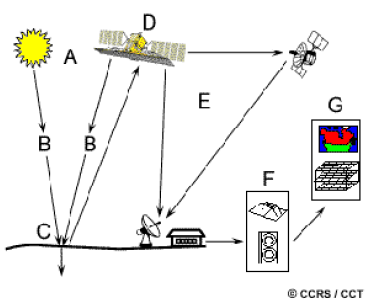
\includegraphics[width=0.4\textwidth]{rs.PNG}
\caption{Aardopservatie \label{fig:rs} Deze afbeelding komt uit \textit{Fundamentals of remote sensing\cite{fun}}}
\end{wrapfigure}


%Het gedetai\"eerde proces verloopt zoals hierna beschreven\cite{fun}, en is te zien in figuur \ref{fig:rs} .

%Een lichtstraal ontstaat aan een zo genaamde lichtbron, wat in de meeste gevallen de zon is. Deze lichtstraal reist door de ruimte en door de atmosfeer, tot deze contact maakt men een materiaal, en hierop een of meerdere keren reflecteert. Daarna reist deze lichtstraal opnieuw door de atmosfeer tot deze contact maakt met een camera op een satelliet. De eigenschappen van deze lichtstraal worden be\"invloed door elk van deze processen.

Aardobservatie begint bij een lichtbron\footnote{In het geval dat men ge\"interesseerd is in het thermisch infrarood spectrum, is er geen lichtbron nodig aangezien materialen op kamertemperatuur van nature dit soort licht uitstralen, ten gevolge van black body radiation.}. Deze lichtbron is vaak de zon, maar dit proces is gelijkaardig voor andere lichtbronnen. De lichtbron zendt een lichtstraal uit, die eerst door de ruimte en vervolgens door de atmosfeer reist, totdat deze contact maakt met een materiaal op het aardoppervlak en hierop een of meermaals reflecteert. Deze reflectie verandert de eigenschappen van de lichtstraal. De gereflecteerde lichtstraal reist opnieuw door de ruimte, totdat deze in contact komt met de detector op een satelliet. Deze detector zet de lichtstraal om in elektrische signalen, die verzonden worden vanaf de satelliet naar het aardoppervlak, waar deze geanalyseerd kunnen worden. Dit volledige proces wordt afgebeeld op figuur \ref{fig:rs}. 



%Elke lichtstraal is een golf in het elektromagnetische spectrum. Deze golf wordt enerzijds bepaald door zijn golflengte, wat de lengte is tussen twee opeenvolgende maxima van de golf, zoals afgebeeld in figuur \ref{fig:golflengte}. Anderzijds wordt de golf bepaald door de intensiteit, wat de grootte is van de piek van de golf. Soms wordt de frequentie van de golf gebruikt om deze te karakteriseren, maar die kan bepaald worden uit de golflengte en de snelheid van het licht. In werkelijkheid is een lichtstraal niet een golf, maar een combinatie van verschillende golven met elk hun golflengte en intensiteit. De bijbehorende intensiteit bij elke golflengte wordt het spectrum genoemd.

\subsubsection{elektromagnetische golven}
Een lichtstraal is een elektromagnetische golf, waarvan een van de belangrijkste eigenschappen voor aardobservatie de golflengte is. Voor een vlakke golf is deze golflengte de afstand tussen twee opeenvolgende cycli, zoals te zien in figuur \ref{fig:rs}. Echter, een lichtstraal is in werkelijkheid bijna nooit een vlakke golf, maar een combinatie van verschillende vlakke golven met verschillende golflengten. De intensiteit van elke vlakke golf voor elke specifieke golflengte wordt het spectrum genoemd. Soms wordt in plaats van golflengte ook frequentie gebruikt, maar deze kan eenvoudig bepaald worden uit de golflengte en de snelheid van het licht.

\subsubsection{hyperspectrale cameras}
Gewone beelden van een camera bevatten drie kleuren, elke passende bij een specifieke golflengte. De keuze voor deze drie kleuren, namelijk rood, groen en blauw, is een gevolg van de beperkingen van het menselijk oog. Dit zijn namelijk de kleuren die een mens kan waarnemen. Om dit beeld digitaal te representeren, moet het beeld opgedeeld worden in kleine, even grote, vierkante elementen, genaamd pixels. Elk van deze pixels bevat voor elke kleur een waarde, die de intensiteit van elke respectievelijke kleur in dit vierkant weergeeft. Hyperspectrale cameras werken in essentie op dezelfde manier, alleen detecteert deze camera niet alleen de hoeveelheid rood, groen en blauw, maar detecteert deze een groot aantal kleuren, genaamd banden. Door het grotere aantal banden vergeleken met een gewone camera, kan hier meer informatie uit gehaald worden. De zon zendt vooral licht uit in het infrarood, zichtbaar licht en ultraviolet en daarom worden er vooral banden gebruikt in dit spectrum, zoals te zien in figuur \ref{fig:specs}.


\begin{figure}
\center
\begin{subfigure}[b]{0.3\textwidth}
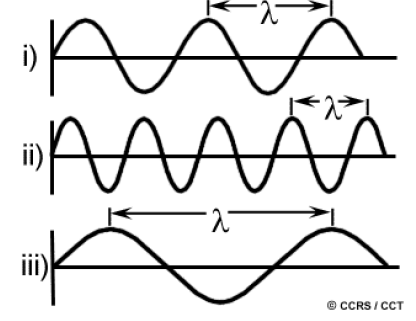
\includegraphics[width=\textwidth]{golflengte.PNG}
\caption{Golven met verschillende golflengten \label{fig:golflengte}}
\end{subfigure} \rulesep
\begin{subfigure}[b]{0.2\textwidth}
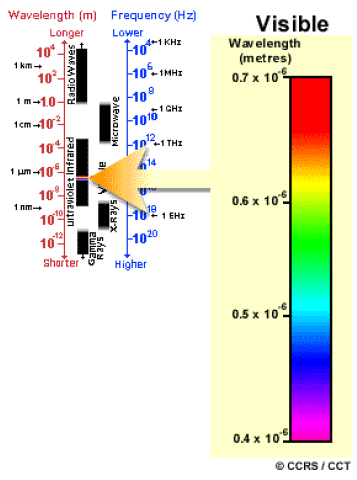
\includegraphics[width=\textwidth]{spec.PNG}
\caption{Het electromagnetische spectrum. \label{fig:spec}}
\end{subfigure}\rulesep
\begin{subfigure}[b]{0.4\textwidth}
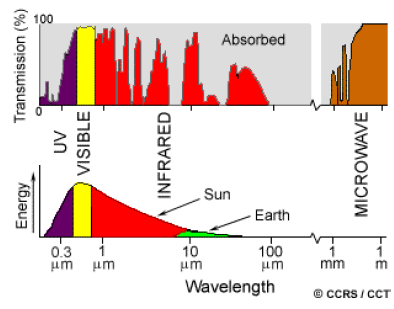
\includegraphics[width=\textwidth]{spec2.PNG}
\caption{Het spectrum van de zon. \label{fig:specs}}
\end{subfigure}
\caption{electromagnetische golven. Deze afbeeldingen komen uit \textit{Fundamentals of remote sensing\cite{fun}}}
\end{figure}


Het doel van spectrale analyse is het bepalen van de hoeveelheden van elk materiaal in een specifieke pixel, gegeven het spectrum van deze pixel. Verschillende methoden hiervoor worden beschreven in deze thesis. 

\section{reflectie} \label{sec:ref}

%Wanneer een lichtstraal invalt op een materiaal reflecteert deze een gedeelte van dit licht. Het nieuwe spectrum van het gereflecteerde licht kan bepaald worden aan de hand van de eigenschappen van het materiaal en het spectrum van het binnenkomende licht. Er kan de benadering gemaakt worden dat de intensiteit voor een gegeven frequentie van het gereflecteerde spectrum alleen afhankelijk is van de intensiteit van het invallende spectrum, en deze daar recht evenredig aan is. In dit geval kan de reflectie beschreven worden als een Hadamard van het spectrum van de inkomende straal en het ``spectrum'' van het materiaal. Dit spectrum is nu geen vector van intensiteiten weer, maar een vector die voor elke frequentie bevat welk deel van de inkomende lichtstraal wordt gereflecteerd. 

Wanneer een lichtstraal invalt op een materiaal reflecteert deze een gedeelte van dit licht en absorbeert deze de rest. Het spectrum van deze lichtstraal dat gereflecteerd noemt men de reflectantie. Dit is afhankelijk van het materiaal en van de golflengte van het licht. 

In deze thesis worden hiervoor drie aannames gemaakt. Ten eerste heeft de gereflecteerde lichtstraal dezelfde golflengte als het invallende licht. Ten tweede is de intensiteit van de gereflecteerde straal recht evenredig met de intensiteit van de invallende straal. Ten derde kan de reflectie van een lichtstraal van een specifieke golflengte niet be\"invloed wordt door licht van andere frequenties. Deze drie aannames zijn correct volgens de klassieke fysica, maar hier zitten correcties op van kwantummechanische effecten. Deze zullen echter klein genoeg zijn zodat ze als deel van de ruis beschouwd kunnen worden.

De intensiteit van de uitgaande straal kan geschreven worden als volgt:

\begin{equation}
E_{out}(\lambda) = R_\lambda E_{in}(\lambda)
\end{equation}

Dit is een stelsel van vergelijkingen (een vergelijking voor elke waarde van $\lambda$, wat overeenkomt met een band in het spectrum). Zowel de intensiteiten als de reflectieco\"efficienten kunnen samengesteld worden tot een vector, en dan geldt

\begin{equation}
\bm{x} = \bm{R}\odot \bm{y}
\end{equation}

met $\odot$ het Hadamard ofwel elementwijs product. De vector $R$ noemt men de reflectie van het materiaal. Deze neemt in beschouwing dat er meerdere interacties kunnen gebeuren in het materiaal. De reflectie waarbij alleen een enkelvoudige interactie meegenomen is noemt men het albedo.


\section{atmosferische correctie}

Wanneer de lichtbron die we beschouwen uniform en genormaliseerd is, is het spectrum van het materiaal gelijk aan het spectrum van het gedetecteerde licht. Alleen is de in werkelijkheid gebruikte lichtbron - meestal is dit de zon - niet uniform. Ook zijn er verschillende effecten die de lichtstraal be\"invloeden\cite{fun} zoals verschuiving, atmosferische verstrooiing, Rayleigh verstrooiing, Mie verstrooiing, nonselectieve verstrooiing, atmosferische absorptie, ozon absorptie, $CO_2$-absorptie en interpixel verstrooiing. De gebruikte datasets in deze thesis zijn door een algoritme gecorrigeerd voor al deze effecten, en de beelden kunnen  deze dus beschouwd worden als verlicht door een uniforme lichtbron, waarbij de gedetecteerde lichtstraal alleen be\"invloed is door reflecties en Gaussische ruis. 

\section{toepassingen}


Een veelgebruikte toepassing van aardobservatie is het in kaart brengen van landbouwgewassen\cite{fun}. Men kan niet alleen het soort gewas op een akker in kaart brengen, maar ook onder andere de gezondheid en verwachte oogst van verschillende gewassen. In het verleden werd het in kaart brengen van gewassen gedaan door steekproeven te nemen met de hand vanop de grond, maar aardobservatie is nauwkeuriger, goedkoper en kan eenvoudiger gestandaardiseerd worden. Enerzijds is deze informatie nuttig voor de landbouwers zelf, omdat deze aan de hand van de data kunnen bepalen welke gewassen het beste groeien op welke plaats en wanneer er het best gezaaid of geoogst wordt. AAn de andere kant is deze informatie ook nuttig voor overheden en verzekeraars, omdat deze kunnen nagaan welke planten er geplant worden,  voorspellen wat de oogst gaat zijn en bepalen wat de schade is na een droogte of storm. 

Aardobservatie wordt ook toepast in de geologie. Van de aardbodem kan niet alleen het soort gesteente aan de oppervlakte in kaart gebracht worden, maar ook de formatie van deze gesteentes en zelfs de gesteentes liggend onder de aardbodem. Een van de voor de hand liggende toepassingen hiervan is de mijnbouw. Een ander toepassing hiervan is voor het voorspellen van aardbevingen, aardverschuivingen en vulkanisme, wat inhoud dat aardobservatie gebruikt kan worden voor het plannen van wegen, gebouwen en andere structuren. 

  
\begin{figure}
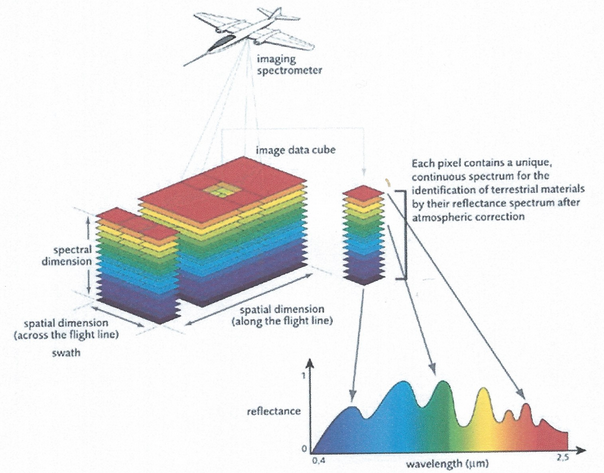
\includegraphics[width=\textwidth]{hyp.PNG}
\caption{Opbouw van een hyperspectraal beeld. Deze afbeelding komt uit \textit{Fundamentals of remote sensing\cite{fun}}}
\end{figure}

\chapter{Spectraal ontmengen}



%Het doel van spectrale anaylise is om uit deze hyperspectrale beelden het bepalen welke materialen zich op een specifieke pixel bevinden. Hoewel het belangrijkste toepassing hiervan de aardopservatie is, kan dit evidenterwijs ook gebruikt worden om materialen te analyseren in een laboratorium of voor bijvoorbeeld kwaliteitscontrole in de industrie.

\section{Resolutie}

Een pixel in een hyperspectraal beeld bevat een of meerdere materialen. Indien elke pixel maar een enkel materiaal zou bevatten, zou elk spectrum van elke pixel vergeleken kunnen worden met een referentiespectrum. Echter, het is theoretisch onmogelijk om een camera te maken met resolutie die groot genoeg is om dit te verwezenlijken. De hoeveelheid licht dat op de camera valt is immers beperkt, en moet verdeeld worden over alle pixels en de verschillende banden. Dit betekent dat wanneer de pixels te klein worden, elke pixel te weinig licht krijgt en de signaal ruis verhouding te laag wordt, en aangezien licht bestaat uit fotonen, is er een limiet van de gevoeligheid van de camera. 

De enige methode om de gevoeligheid te verhogen is bijgevolg een langere belichtingstijd. Dit zorgt echter voor een vergroting van de ruis en is niet haalbaar voor een satelliet in een baan rond de aarde - zelfs als het praktisch haalbaar was om de resolutie kleiner te maken, ligt het probleem vooral in de fractalische eigenschappen van vele objecten. 

Als er bijvoorbeeld in een bos een zeer grove resolutie gebruikt wordt, vallen er verschillende soorten bomen in een enkele pixel. Als de pixels kleiner worden, kunnen bomen al van elkaar onderscheiden worden, maar de takken van verschillende bomen nog niet. Zelfs een blad bestaat nog uit verschillende materialen, aangezien de nerven van het blad uit ander materiaal bestaan dan de bladmoes. Ook bij mineralen heeft men hetzelfde probleem: een gesteente bevat verschillende mineralen, maar om deze van elkaar te kunnen onderscheiden moet de pixelgrootte op microscopisch niveau zijn. 

Hierom is het van belang om een spectra van een pixel, dat een combinatie is van de spectra van de verschillende materialen in deze pixel, te kunnen ``ontmengen''. Hierbij is men specifiek ge\"interesseerd in de abundantie van elk materiaal: een getal dat het gedeelte van de lichtstralen dat afkomstig is van dat specifiek materiaal in een pixel weergeeft. Aangezien dit een goede maat is voor de aanwezige hoeveelheid van een bepaald materiaal in een pixel, is dit de belangrijkste parameter.

\section{Spectrale analyse}

Het spectrum van licht kan beschreven worden als een wiskunde functie die een frequentie omzet in een intensiteit. In werkelijkheid bevat een hyperspectraal beeld niet de volledige functie, maar bevat deze tweehonderd waarden in deze functie, de zogenoemde banden. In matlab\citep{MATLAB} zal dit worden opgeslagen als een driedimensionale tensor, waarbij de verschillende assen de x positie, y positie en de band van de pixel weergeven. 

In deze thesis is men niet ge\"interesseerd in  interpixel-interacties, wat betekent dat het materiaal in een pixel geen invloed heeft op het spectrum van andere pixels. Correcter zegt dit dat de materialen in een enekel pixel niet meer invloed hebben op naastliggende pixels dan op andere willekeurige pixels in dit beeld. Daardoor is de exacte structuur van de pixels niet van belang en kan deze worden vervangen door een lijst van pixels die elk afzonderlijk ontmengd moeten worden.  Bijgevolg kan de drie-dimensionale tensor worden omgezet in een matrix, waar de rijen de verschillende pixels zijn en de kolommen de banden.  


%\begin{itemize}
%\item spectra als functies (eigenschappen van licht)
%\item spectra als vector (endmembers) $\rightarrow$ matlab implementatie
%\item mengen van endmembers (abundancies)
%\end{itemize}




\section{Lineair ontmengen}

Bij lineair ontmengen wordt uitgegaan van het ``lineair mixing model''. Een lichtstraal valt in in een pixel op een enkel wel bepaald materiaal, interageerd met dit materiaal een enkele keer, en valt dan op de detector. Dit betekend dat het spectrum van de teruggekaatste lichtstraal alleen afhangt van de reflectantie van dit materiaal, de endmember genaamd. De totale reflectantie van een pixel die gemeten wordt is een gewogen gemiddelde van deze verschillende endmembers, waarvan het gewicht van elke endmember bepaald wordt door het gedeelte van de lichtstralen dat op dit materiaal gereflecteerd wordt. Dit gedeelte is de abundantie. In symbolen geeft dit:


% waarbij uitgegaan wordt dat elke lichtstraal die op een pixel valt enkelvoudig reflecteert en daarna op de detector valt. Het totale spectra op de detector is het gewogen gemiddelde van de spectra van de verschillende endmembers, waarbij het gewicht voor elke endmember de abundantie is van deze endmember. Men krijgt volgende uitdrukking: 


\begin{align}
\bm{x} &= \sum_i a_i \bm{e}_i \label{eq:nq}
\end{align}

Waarbij $\bm{x}$ het gemeten spectrum is, $e_i$ de endmembers en  $a_i$ de abundanties.
Echter, omdat het mixing model slechts een benadering is van de werkelijkheid en omdat op een experimentele meting altijd een vorm van ruis zit, kan het exacte spectrum nooit gevonden worden. Er wordt daarom gezocht naar het reconstructiespectrum dat het dichtst ligt bij het werkelijke spectrum. De ruis wordt verondersteld normaal verdeeld te zijn. Dit is een eenvoudig gevolg van het centrale-limiet theorema, dat zegt dat de som van een groot aantal kansvariabelen normaal verdeeld is. 

Noem $\bm{x}$ het gemeten spectrum, en $\bm{y}$ het reconstructiespectrum, met $\bm{\eta}$ de ruis, dan is

\begin{equation}\label{eq:rec0}
\bm{x} = \bm{y} + \bm{\eta}
\end{equation}

De kans dat $\bm{x}$ gemeten wordt, gegeven dat $\bm{y}$ het werkelijk gemeten spectrum is, is $f(\eta)$, waarbij $f$ de normale verdeling is. Aangezien de normale verdeling alleen afhankelijk is van de kwadratische norm, zijn we ook alleen ge\"intereseerd in de kwadratische norm van de ruis. De normale verdeling is ook groter wanneer deze kwadratische norm kleiner is, dus moet om de kans te maximaliseren de norm van de ruis geminimaliseerd worden. 

Deze norm kan berekend worden gebruik makend van vergelijking \ref{eq:rec0}.

\begin{eqnarray}
\left|\bm{\eta}\right| &= \left|\bm{x} - \bm{y}\right| \label{eq:rec}
\end{eqnarray}

De uitdrukking $\left|\bm{x} - \bm{y}\right|$ noemt men de reconstructie-error. Het is deze uitdrukking dat geminimaliseerd moet worden bij ontmenging. 


\subsection{Minimaliseren van reconstructieerror}
Voor het linair model wordt in dit hoofdstuk er vanuit gegaan dat de endmembers gekend zijn, maar de abundanties en de ruis niet. Als de ruis wordt toegevoegd aan vergelijking \ref{eq:nq} dan geldt:

\begin{align}
\bm{x} &= \sum_i a_i \bm{e}_i + \eta
\end{align}

Het minimaliseren van de reconstructie-error, gebruik makend van vergelijking \ref{eq:rec}:

\begin{align}
\text{argmin}_{a_1 ... a_p} \left| \bm{x} - \sum_{i=1}^p a_i \bm{e}_i\right|^2
\end{align}

Indien de abundanties $a_i$ vrije re\"ele waarden zouden zijn, zou dit minimum eenvoudig berekend kunnen worden, door een projectie te nemen opgespannen door het vlak van de endmembers. Deze projectie kan genomen worden als volgt. Neem $E = [e_1,e_2,...,e_n]$ een matrix met als kolommen de verschillende endmembers. De projectie op de deelruimte opgespannen door de elementen van $E$ kan gevonden worden aan de hand van de Penrose-inverse matrix.

\begin{equation}
\bm{a} = (E^T E)^{-1} E^T \bm{x}
\end{equation}

Doordat de abundanties een gedeelte van lichtstralen zijn dat op een materiaal botst, zijn er twee extra voorwaarden hierop. Enerzijds moeten de abundanties positief zijn, aangezien men geen negatieve hoeveelheid lichtstralen kan hebben. Dit noemt men de niet-negativiteitsvoorwaarde. Anderzijds kan elke lichtstraal maar op een enkel materiaal botsen, dus is de som van alle gedeeltes \'e\'en. Dit noemt de eenheidssomvoorwaarde.  


\subsubsection{niet-negativiteit}

De niet negativiteitsvoorwaarde geeft weer dat de abundanties allemaal positief moeten zijn, of met andere woorden groter moeten zijn dan nul. Dit betekend dat men niet moet projecteren op de deelruimte, maar op een deelverzameling hiervan. Hiervoor kan een aangepast algoritme gebruikt worden, namelijk het ``nonnegative least-squares curve fitting'' of\texttt{lsqnonneg} algoritme, maar dit algoritme is veel berekeningsintensiever dan het penrose-inverse algoritme. Later in sectie \ref{sec:select} wordt een alternatieve methode beschreven om met deze voorwaarde om te gaan.

\subsubsection{eenheidssom}

De eenheidssomvoorwaarde geeft weer dat de abundanties moeten sommeren tot \'e\'en. Dit zorgt ervoor dat de mogelijke abundanties geen deelruimte meer opspannen, aangezien het nulpunt geen deel meer is van het hypervlak. Dit kan worden opgelost door een van de endmembers als shadow te beschouwen. Dit houdt in dat het hypervlak verschoven wordt over de vector $e_1$ zodanig dat het nulpunt deel wordt van de hyperruimte en dit terug een deelruimte is.

Deze transformatie houdt in dat de matrix $E$ getranslateerd wordt naar $[e_2-e_1;e_3-e_1;...;e_n-e_1]$ en het gemeten spectrum naar $\bm{x} - e_1$. Na deze transformatie kan het Penrose-inverse algoritme worden toegepast, zodat men de abundanties $a_2,a_3,...,a_n$ krijgt. De laatste abundantie $a_1$ kan gevonden worden door de eenheidssomvoorwaarde te eisen, zodat $a_1 = 1 - \sum{i=2}^{n} a_i$.

\vspace{5 mm}
Het algoritme dat beide bovenstaande correcties doorvoert noemt men het ´´fullyconstrained
least-squares unmixing model''. Het algoritme dat enkel de eenheidssomvoorwaarde meeneemt, maar niet de nietnegativiteisvoorwaarde, noemt men het ´´sum-to-one''
constrained least-squares unmixing model''.


 
\vspace{5 mm}

Volgende secties beschrijven twee belangrijke problemen voor spectraal ontmengen, en hiervoor wordt een oplossing beschreven in de rest van deze thesis.


\section{Niet-linaire interacties}

In vorig hoofdstuk is men ervan uitgegaan dat elke lichtstraal maar een enkele keer interageert met een enkel materiaal. Dit is een goede benadering wanneer men vlakke gebieden met duidelijk verdeelde endmembers beschouwd. Echter, dit geldt niet meer voor geometrische structuren zoals gebouwen of vegetatie, waarbij enkelvoudige interacties zeldzaam zijn en de meerderheid van de lichtstralen meermaals interageert. Hetzelfde geldt voor gebieden met mineralen, waarbij lichtstralen meerdere keren interagerend met een enkele korrel en effecten zoals transmissie belangrijk worden.

In deze thesis wordt er geen rekening gehouden met transmissie-effecten en interpixelinteracties. Dit laatste is het fenomeen waarbij een lichtstraal interageerd met materialen in twee of meer verschillende pixels. Wel wordt er rekening gehouden met niet-linaire effecten in een enkele pixel, wat inhoud dat een lichtstraal meerdere keren kan interageren met dezelfde of verschillende materialen in een enkele pixel. Hiervoor bestaan er twee veelgebruikte modellen, namelijk het bilinair en het multilinair model.

\section{Variabiliteit}\label{sec:select}

In dit hoofdstuk werd ervan uitgegaan dat elke endmember een enkel vast spectrum heeft. In werkelijkheid is dit niet het geval. Enerzijds worden verschillende materialen vaak beschouwd als een enkel materiaal. Bijvoorbeeld de bovenkant en de onderkant van een blad hebben een verschillend spectrum. Ook door de mens gemaakte materialen, zoals beton en asfalt, kunnen verschillende spectra hebben. Meestal is het niet interessant om een onderscheid te maken tussen deze verschillende materialen. Anderzijds kan het spectrum van een enkel materiaal ook verschillen dankzij verschillen in belichting en atmosfeer. Deze beide effecten zorgen ervoor dat een enkele endmember meerdere spectra kan hebben. Dit concept noemt variabiliteit. Dit betekend dat elke endmember beschreven wordt door een bibliotheek van spectra, in plaats van een enkel spectrum. Hoe kan worden ontmengd rekening houdend met variabiliteit staat beschreven in sectie \ref{sec:mesma}. 

\section{Vrijheidsgraden} \label{sec:vrij}

In een optimalisatieprobleem noemt men het aantal re\"ele continue variabelen waarvan een variabele afhankelijk is de vrijheidsgraden. Wanneer het aantal te bepalen vrijheidsgraden groter is dan het aantal gegeven vrijheidsgraden, dan is het probleem ondergedefini\"eerd. Dit houdt in dat er meerdere mogelijke oplossingen voor de vrije parameters zijn waarvoor alle voorwaarden voldaan zijn. Als dit voorkomt, is een gevonden oplossing niet met zekerheid de juiste oplossing, en geeft het model dus verkeerde oplossingen terug, die lijken te voldoen aan het systeem.

Het aantal vrijheidsgraden van het gemeten spectrum is per definitie het aantal banden van de gebruikte sensor. Bij de Avari sensor, welke gebruikt is voor de beelden in dit verslag, is dit $200$. Maar uit dimensionale analyse volgt dat het werkelijke aantal vrijheidsgraden maar rond de $15$ ligt. Als er dus een model gebruikt wordt met meer dan $15$ parameters geeft dit per definitie een goed resultaat, zelfs als dit model totaal niet overeenkomt met de werkelijkheid. Wanneer verschillende modellen vergeleken worden, zal een model met meer vrijheidsgraden een lagere reconstructie-error hebben. 

\chapter{Niet-lineariteit en endmember variabiliteit} 

\section{Bilinair ontmengen}

Het bilineair model beschrijft dat elke lichtstraal \'e\'en of twee keer kan reflecteren. Van dit model bestaan twee varianten. Enerzijds bestaat het model van Nascimento en Somers\cite{mlinmix}. Deze voegt de bilinaire term is als volgt.

\begin{equation}
\bm{x} = \sum a_i \bm{e}_i + \sum a_i a_j \bm{e}_i \odot \bm{e}_j + \bm{\eta}
\end{equation}

Deze geeft in de praktijk geen goede resultaten, omdat het bilinair model is ontwikkeld voor objecten met een ingewikkelde geometrie, en dat deze methode echter geen parameters of informatie bevat over deze geometrie. Dit probleem kan worden opgelost door gebruik te maken van het Fan model\cite{mlinmix}, dat beschrijft dat de endmembers worden gemengd als volgt:

\begin{equation}
\bm{x} = \sum a_i \bm{e}_i + \sum \gamma_{ij} a_i a_j \bm{e}_i \odot \bm{e}_j + \bm{\eta}
\end{equation}

Dit model heeft een ander probleem, namelijk dat voor een model met $p$ materialen, dit model $p^2$ extra vrijheidsgraden bevat. Dit betekend dat er geen garantie is dat het model het juiste resultaat weergeeft, zoals beschreven in sectie \ref{sec:vrij}. 

Wegens deze problemen met het bilinaire model, wordt er overgegaan naar het multilinair model dat sterker fysisch onderbouwd is, en dat meer dan twee reflecties meeneemt. Dit model wordt beschreven volgende sectie.

\section{multilineair ontmengen} \label{sec:multi}

Het multilinair model gaat ervan uit dat een lichtstraal meerdere kan reflecteren in een enkele pixel. Dit model is gebaseerd op \textit{A multilinear mixing model for nonlinear spectral unmixing}\cite{mlinmix}. 

\begin{wrapfigure}{R}{0.4\textwidth}
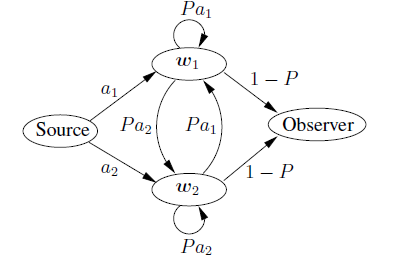
\includegraphics[width=0.4\textwidth]{multi.PNG}
\caption{Markov-ketting van het multilineair model \label{fig:multi}}
\end{wrapfigure}

De inkomende lichtstraal valt in op een materiaal binnen een pixel. Wanneer deze invalt op het materiaal heeft deze een kans $P$ om opnieuw in te vallen op hetzelfde of een ander materiaal in dezelfde pixel, en een kans $(1 - P)$ om te reflecteren naar de detector. De kans voor de gereflecteerde lichtstraal om in te vallen op een specifiek materiaal is gelijk aan diezelfde kans voor een lichtstraal afkomstig van de bron, namelijk de abundantie van de materiaal. Het spectrum van de lichtstraal veranderd bij elke interactie zoals beschreven in sectie \ref{sec:ref}. Dit wil zeggen dat de uitgaande lichtstraal  het elementwijs product is van de invallende lichtstraal en het albedo van het materiaal.
Dit hele proces kan worden voorgesteld als een Markov-ketting zoals te zien in figuur \ref{fig:multi}.

%\begin{enumerate}
%\item De inkomende straal interageert met minstens \'e\'en materiaal in de bron.
%\item Na deze interactie heeft het materiaal een kans $P$ om een nieuwe interactie aan te gaan, en een kans $(1-P)$ om dat niet te doen.
%\item De kans om een nieuwe interactie aan te gaan met elk nieuw materiaal is evenredig met de abundantie van dat materiaal. Merk op dat aangezien de som van de abundaties \'e\'en is, de waarde van de kans gelijk is aan de abundantie.
%\item Wanneer een lichtstraal interageert met een materiaal wordt zijn spectrum gewijzigd, afhankelijk van het albedo van dit materiaal.
%\end{enumerate}

\subsection{berekening}

In deze sectie nomen we het "pad" van een lichtstraal de verzameling van de verschillende endmembers waarop het materiaal reflecteert, waarbij er rekening wordt gehouden met de volgorde. De kans dat een welbepaald pad gevolgd wordt, wordt als volgt genoteerd:

\begin{equation}
\mathcal{P}(i_1,i_2,i_3,...,i_R)
\end{equation}

Met andere woorden, deze uitdrukking geeft de kans weer dat een lichtstraal reflecteert op materiaal $i_1$, daarna op $i_2$, op $i_3$ en zo voort, totdat deze uiteindelijk interagerend met materiaal $i_R$. $R$ is hier het totale aantal materialen waarop gereflecteerd wordt.

De kans op dit pad kan worden uitgerekend aan de hand van het voorgenoemde Markov-proces\cite{mlinmix}. 

\begin{equation}
\mathcal{P}(i_1,i_2,i_3,...,i_R) = P^{R-1} (1-P) \prod_{k=1}^R a_{i_k}
\end{equation}

Het spectrum van de uitgaande straal ten gevolge van een specifiek pad is $\Odot_{k=1}^R \bm{w}_{i_k}$, waarbij $\bm{w}_{i_k}$ het albedo is van materiaal $i_k$, en $\Odot$ het elementwijsproduct. Aan de hand hiervan kan de bijdrage van een specifiek pad, wat de kans vermenigvuldigt met het spectrum is, berekend worden als volgt:
\begin{equation}
\bm{x}_{(i_1,i_2,i_3,...,i_R)} = P^{R-1} (1-P) \Odot_{k=1}^R \left(a_{i_k} \bm{w}_{i_k}\right)
\end{equation}

Gesommeerd over alle mogelijke paden geeft dit het totale gemeten spectrum. Deze som over alle paden kan berekend worden door de som te nemen over alle mogelijke waarden van $R$ voor een enkel pad, en dan als $R$ -wat hier betekend het aantal interacties- gekend is, kan voor elke interactie gesommeerd worden over alle materialen. Wanneer alle bijdragen van elk pad gesommeerd zijn over alle paden, geeft dit het totale spectrum terug dat de detector meet, en dit is gelijk aan:

\begin{equation}
\bm{x} = \sum_{R=1}^{\infty} \left(\sum_{i_1}^{p} ... \sum_{i_R}^{p}\right)P^{R-1} (1-P) \Odot_{k=1}^R \left(a_{i_k} \bm{w}_{i_k}\right)
\end{equation}

Stel dat de kans dat een lichtstraal nog een keer interageerd afhankelijk is van het materiaal. De kans dat een specifiek pad gevolgd wordt is kan op analoge wijze worden berekend

\begin{align}
\mathcal{P}(i_1,i_2,i_3,...,i_R) &= \prod_{k=1}^{R-1}P_{i_k} (1-P_{i_R})\\
&= \prod_{k=1}^{R}P_{i_k} \frac{1-P_{i_R}}{P_{i_R}}
\end{align}
Waarbij $P_{i_k}$ de reflectiekans van materiaal $i_k$ is. 

De spectrum dat gemeten wordt afkomstig van een specifiek pad wordt nu:

\begin{align}
\bm{x}_{(i_1,i_2,i_3,...,i_R)} &= \prod_{k=1}^{R-1}P_{i_k} (1-P_{i_R}) \Odot_{k=1}^R \left(a_{i_k} \bm{w}_{i_k}\right) \\
&= \Odot_{k=1}^{R-1} \left(P_{i_k}a_{i_k} \bm{w}_{i_k}\right) \odot (1-P_{i_R}) a_{i_R} \bm{w}_{i_R} \\
\bm{x} &= \sum_{R=1}^{\infty} \left(\sum_{i_1}^{p} ... \sum_{i_R}^{p}\right) \Odot_{k=1}^{R-1} \left(P_{i_k}a_{i_k} \bm{w}_{i_k}\right) \odot (1-P_{i_R}) a_{i_R} \bm{w}_{i_R} \\
&= \sum_{i=1}^p (1-P_i) a_{i} \bm{w}_{i} + \sum_{i=1}^p \sum_{j=1}^p (1-P_i) a_{i} \bm{w}_{i} \odot P_j a_{j} \bm{w}_{j} \nonumber\\&+ \sum_{i=1}^p \sum_{j=1}^p \sum_{k=1}^p (1-P_i) a_{i} \bm{w}_{i} \odot P_j a_{j} \bm{w}_{j} \odot P_k a_{k} \bm{w}_{k} \nonumber\\&+ \sum_{i=1}^p \sum_{j=1}^p \sum_{k=1}^p  \sum_{l=1}^p (1-P_i) a_{i} \bm{w}_{i} \odot P_j a_{j} \bm{w}_{j} \odot P_k a_{k} \bm{w}_{k} \odot P_l a_{l} \bm{w}_{l} \nonumber \\& + ... \\
&= \bm{z} + \bm{y}\odot\bm{z} + \bm{y}\odot\bm{y}\odot\bm{z} + ... \\
&= \bm{z} + \bm{y}\odot\bm{x} \\
 &= \frac{\bm{z}}{1-\bm{y}}
\end{align}
waar
\begin{align}
\bm{y} &= \sum_{i=1}^p P_i a_{i} \bm{w}_{i} \\
\bm{z} &= \sum_{i=1}^p (1-P_i) a_{i} \bm{w}_{i} 
\end{align}
zodat
\begin{equation}
\bm{x} = \frac{\sum_{i=1}^p (1-P_i) a_{i} \bm{w}_{i}}{1-\sum_{i=1}^p P_i a_{i} \bm{w}_{i}} \label{eq:Pi}
\end{equation}

Dit is een uitdrukking voor het multilineair mengen van endmembers waarbij de reflectiekans endmember afhankelijk is. Indien men ge\"intereseerd is in een onafhankelijke reflectiekans, kan de formule hiervoor bekomen worden door te stellen dat $P_i = P \forall i$ zodat het reconstructiespectrum wordt:

\begin{equation}
\bm{x} = \frac{(1-P) \sum_{i=1}^p a_{i} \bm{w}_{i}}{1-P\sum_{i=1}^p  a_{i} \bm{w}_{i}} \label{eq:P}
\end{equation}

wat exact overeenkomt met de formule in de literatuur\cite{mlinmix}.

Om aan de hand van dit model te ontmengen moet nog steeds gebruik gemaakt worden van het minimaliseren van de reconstructie-error. 

\begin{align}
\text{argmin}_{a_1 ... a_p; P_1 ... P_p} \left| \bm{x} - \frac{\sum_{i=1}^p (1-P_i) a_{i} \bm{w}_{i}}{1-\sum_{i=1}^p P_i a_{i} \bm{w}_{i}} \right|^2
\end{align}

Aangezien deze vergelijking niet lineair is en dus ook geen hypervlak opspant, kan deze uitdrukking niet geminimaliseerd worden door middel van projecties, en zijn hier geavanceerde minimalisatietechnieken voor nodig. In matlab\cite{MATLAB} wordt voor deze thesis hier de functie \texttt{fmincon} gebruikt. Deze neemt gewoon de uitdrukking $\left| \bm{x} - \frac{\sum_{i=1}^p (1-P_i) a_{i} \bm{w}_{i}}{1-\sum_{i=1}^p P_i a_{i} \bm{w}_{i}} \right|^2$ in en geeft hier een minimum voor terug. Dit heeft als nadeel dat het draaien van deze functie op de experimentele data later beschreven in deze thesis een looptijd heeft van ongeveer $0.1$ seconden voor elke pixel, in tegenstelling tot het berekenen van pseudo-inversen, wat ongeveer $50$ microseconden in beslag neemt. 

\subsection{reflectancy vs albedo}

Het albedo  $\bm{w}_i$ uit vorig hoofdstuk kan in werkelijkheid niet exact gemeten worden. In theorie kan deze afgeleid worden uit de reflectie van een meting met een enkele endmember. Dit kan bepaald worden door vergelijking \ref{eq:Pi} te inverteren, zodat:

\begin{equation}
\bm{w}_i = \frac{\bm{e}_i}{\bm{e}_iP_i + 1 - P_i}
\end{equation}
Waarbij de deling de elementwijze deling is. 

Het probleem hierbij is dat hier wordt verondersteld dat $P_i$ gekend is, wat in werkelijkheid niet het geval is. Daarom wordt vaak verondersteld dat $P_i \approx 0$ wat neerkomt op een benadering die stelt dat $\bm{w}_i \approx \bm{e}_i$. 

\subsection{Ondergrens van P waarde}

$P$ is per definitie een getal groter dan nul, omdat kansen tussen nul en een liggen. Echter, het is mogelijk om in vergelijking \ref{eq:Pi} een negatieve waarde in te voeren. Deze waarde kan in werkelijkheid negatief zijn ten gevolge van twee fysische situaties. Enerzijds is, zoals beschreven in de vorige sectie, het albedo slechts een benadering. Doordat de reflectie van de referentie-endmember nul wordt verondersteld te zijn, is deze lager dan werkelijkheid. Bijgevolg zal ook de $P$ waarde van de pixel lager zijn dan in de werkelijkheid. In het geval de reflectiekans van de pixel lager is dan de reflectiekans van het referentiemateriaal, zal deze waarde zelfs onder nul liggen. Merk op dat dit systeem niet linair is, waardoor een verkeerde reflectiekans van bovengenoemde sectie niet kan opgelost door het herdefini\"eren van $P$. Anderzijds zijn er ook interpixelinteracties die invloed hebben op het systeem. Deze kunnen extra lichtstralen die al hebben gereflecteerd op het materiaal toevoegen aan het systeem, wat zorgt voor een verlaging van de reflectiekans. 

%\subsection{afhankelijke vs onafhankelijke P waarden}





\section{MESMA} \label{sec:mesma}

\begin{itemize}
\item Ontmengen aan de hand van elke subset
\item Selectie op basis van niet-negativiteitsvoorwaarde
\end{itemize}

\subsection{ontmengingsmethode naar keuze (lineair vs multilineair)}

\section{AAM}

\begin{itemize}
\item concept hoek in hoogdimentonale ruimtes
\item AAM
\end{itemize}


\chapter{Variabiliteit voor niet-lineaire systemen.}

\section{Semi-lineair model}

ontkoppeling van Ontmenging in MESMA bij selectie tov ontmenging voor abundancies

\subsection{Theoretische controle dmv monte carlo simulaties}

\section{multilineair AAM}

\chapter{experimentele vergelijking van verschillende methodes}

\section{looptijd en reconstructie-error}

\section{Alina dataset}

\section{Lijst en korte uitleg bij alle methodes}

Elke methode is hiervoor beschreven, maar dit beschrijft kort de verschillen in de methodes en hoe deze ge\"implementeerd zijn door middel van `schakelaars' in de code. Ook een uitleg bij de weergave van de resultaten. 

\begin{itemize}
\item lineair MESMA
\item semi-lineair MESMA
\item multi-lineair MESMA
\item lineair AAM
\item multilineair AAM
\end{itemize}

$\rightarrow$ Voor de multilineaire modellen wordt ook al dan niet $P> 0$ en $P$ materiaalafhankelijk vergeleken.



\section{Bepreking lineair vs semi-linair}

Verschil voor hoge reflectie (bomen)
$\rightarrow$ semilinair geeft betere resultaten voor dezelfde runtime

\section{Bespreking semi-lineair vs multilineair}

$\rightarrow$ semilineair geeft vergelijkbare resultaten op kortere tijd

\section{Bespreking P-afhankelijkheid}

$\rightarrow$ P-afhankelijkheid geeft vergelijkbare resultaten op gelijke tijd, maar heeft meer vrijheidsgraden

\section{Bespreking P-ondergrens}

verschil voor lage reflectie (asfalt)
$\rightarrow$ Weglaten van ondergrens geeft betere resultaten op gelijke tijd.

\section{Bepreking multilinair AAM vs semilinair model}

$\rightarrow$ zelfde resultaten voor kortere tijd.

\begin{appendices}


\end{appendices}


\begin{flushleft}
\nocite{*}
\bibliography{biblio}{}
\bibliographystyle{plain}
\addcontentsline{toc}{chapter}{Bibliografie}

\end{flushleft}


\end{document}
